Go~\cite{go} is a statically typed language initially developed by Google.
%
It employs channel-based Hoare's Communicating Sequential Processes (CSP)~\cite{hoare-csp78} semantics in its core and provides a productivity-enhancing environment for concurrent programming.
%
Go enjoys accelerating acceptance in a wide variety of
communities including container software systems~\cite{merkel2014docker,kubernetes},  distributed key-value databases~\cite{etcd,cockroachdb-sigmod20}, and web server libraries \cite{grpc}.
%
It involves shared memory, message passing, non-deterministic message reception and selection, dynamic process creation, and programming styles that tend to create thousands of \textit{goroutines}~(\ie,~application-level threads) and discard them to be garbage collected when they reach their final state.
%
The combination of these features is well known for Go's popularity, yet they also make Go challenging to debug.
%
Our work is especially relevant considering that there are no widely practical tools for debugging concurrent Go; even well-curated
concurrency bug benchmark suites are only just now beginning to appear~\cite{tu-concurrentBugs-asplos19,yuan-gobench-cgo21}.
%

In general, concurrent bugs are notoriously difficult to find and reproduce due to the non-deterministic choices that the scheduler makes during execution.
%
In Go, constructs like \textit{select} and buffered channels entangle the process of debugging by introducing extra randomness to the dynamic behavior of the program.
%
Recent static~\cite{ng-dl-cc16,stadtmuller-minigo-aplas16,lange-fence-popl17,lange-staticType-icse18} and dynamic~\cite{go-race-blog,zhao-occam97,sulzmann-corr17,sulzmann-twophase-2018,dilley-gomela-corr2020} techniques have been proposed to address these challenges.
%
GoBench \cite{yuan-gobench-cgo21} gathers a collection of real concurrency bugs (GoReal) and simplified bug kernels (GoKer) from top 9 open-source projects written in Go and evaluated the effectivness such techniques in detecting the bug collection.
%
Although static methods are proved to be rigorously effective in detecting flaws in small programs, they are not practical for realistic programs and often produce false positives.
%
On the other hand, dynamic analysis approaches cover a more significant subset of real-world programs by constructing and analyzing an \textit{execution model}.
%
However, they focus on a specific class of bugs based on the symptom or cause of the bug.
%
Also, for large codebases with thousands of LOC, it is non-trivial to capture an accurate dynamic execution model using source instrumentation or source-to-source translation.
%
Furthermore, our experiments (section \ref{sec:evaluation}) observe that some buggy programs take more than 1,000 runs under different schedules before the bug is hit.
%
Concurrent testing methods~\cite{arora-concrrentTesting-16} are proposed to complement static and dynamic approaches in tackling challenges of concurrent debugging.
%
To the best of our knowledge, there exist no such testing methods applicable to Go.
%

\begin{figure*}[]
\centering
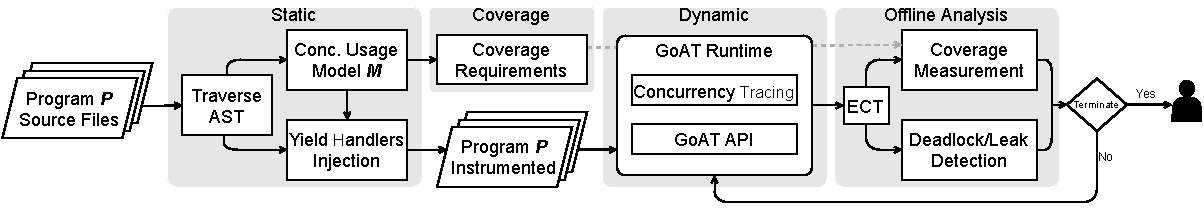
\includegraphics[width=0.99\linewidth]{figs/GOAT_overview.pdf}
%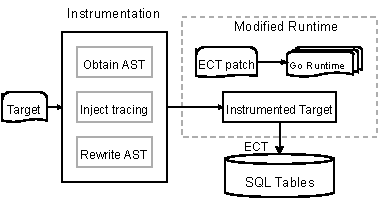
\includegraphics[]{figs/overview.png}
%\includegraphics[]{figs/overv}
\caption{\goat Overview}
\label{fig:goat_workflow}
\end{figure*}


We implemented \goat (\textbf{Go} \textbf{A}nalysis and \textbf{T}esting), a debugging framework for concurrent Go applications to address this lack.
%
\goat (figure \ref{fig:goat_workflow}) combines static and dynamic approaches to automatically analyze the behavior of concurrent components and facilitate the process of testing and debugging Go applications.
%
%We evaluated \goat and compared it against similar tools on the recent Go concurrent bug benchmark~\cite{yuan-gobench-cgo21}.
%
Several classic ideas from literature are combined with novel ones to support modern concepts of Go in \goat, which pursues three primary objectives:
\\
\noindent{\bf Objective 1:\/} \textit{Accurate Dynamic Execution Modeling}---
In order to study the behavior of concurrent components and track the state of the program during execution, a dynamic execution model has to be constructed and compared against a predefined model (e.g., formally defined specifications or the developer's mental representation of the program).
%
It is crucial for debuggers and software analysis tools to construct their execution models as close as possible to the actual program execution context.
%
Since a bug might occur at various levels of abstraction, \textit{whole-program dynamic tracing} provides a practical and uniform way to track multiple facets of the program during execution~\cite{difftrace}.
%
We have enhanced the built-in tracing mechanism of Go~\cite{ect-arxiv} to capture the dynamic behavior of concurrency primitives in the form of a \textit{sequence of events}, namely \textit{execution concurrency trace} or ECT.
%
Each event in ECT represents an \textit{action} that corresponds to exactly one statement in the source code.
%
An ECT provides a detailed model of how a concurrent program behaves dynamically and assists debugging procedures (e.g., bug detection, root-cause analysis, execution visualization).
%
Our experiments show that by replaying the program's ECT, \goat detects all blocking bugs of GoKer~\cite{yuan-gobench-cgo21} many of which are undetected by existing debugging tools.
\\
\noindent{\bf Objective 2:\/} \textit{Systematic Exploration of Schedule-Space}---
Since the scheduler's non-deterministic behavior is the primary reason for Heisenbugs (\ie, errors that are uncommon to occur and hard to reproduce), these bugs may not manifest during conventional testing.
%
By adopting ideas from \textit{systematic concurrency testing} approaches~\cite{dpor,thomson-concurrencyTesting-ppopp14,emmi-delayBounded-popl11,burckhardt-depthBug-asplos10,madanlal-preemptionBound-pldi07,yu-maple-oopsla12,joshi-calfuzzer,contest-jgi01,edelstein2003contest,hong-syncTesting-issta12,christakis-erlang-icst13,yuan-morpheus-asplos20}, we perturb the native scheduler of Go to explore the unconventional but feasible execution interleaving.
%
First, we statically identify the source location of concurrency primitive usages in a given program.
%
We then inject handlers of context-switching calls around these locations to manage schedule perturbation.
%
At its simplest form, handlers randomly (with a certain probablity and within a bound) decide if the current goroutine should continue executing or \textit{yield} to other goroutines to execute first.
%
Such yields change the blocking behavior of the program within the space of feasible states and exercise untested interleavings, consequently heighten the propensity for bug detection.
%
The results of our experiments indicate that just a few random schedule perturbations can accelerate the exposure of rare bugs.

\noindent{\bf Objective 3:\/} \textit{Testing Quality Measurement}---
A test suite's thoroughness is often judged by the coverage of certain aspects of the software, such as its source-code statements (a higher statement coverage indicates more thorough testing).
%
In the context of concurrent software, exisiting coverage metrics~\cite{edelstein2003contest,trainin-followsCoverage-padtad09,hong-syncTesting-issta12,yu-pset-isca09} characterize (quantify) the behavior of concurrency primitives which enables the quality measurement of schedule-space exploration.
%
Such characterizations involve defining an initial set of requirements and a method for assessing whether or not those requirements are met during testing.
%
Since Go combines traditional synchronization and serialization primitives~(mutex, conditional variables) with message-passing and introduces new concepts such as \textit{select-case}~(non-deterministic communication and synchronization), new coverage requirements are required to characterize the behavior of Go concurrency.
%
Using the \goat's infrastructure, we studied the underlying causes of bugs in GoKer benchmark~\cite{yuan-gobench-cgo21} and proposed a set of coverage requirements that 1) coherently characterize the dynamic behavior of concurrency primitives under various scheduling scenarios and 2) enable measurement of schedule-space exploration until reaching a threshold, or exposing the bug.
%
By analyzing the test's ECT, we can identify if coverage requirements are met during testing.
%
We demonstrate that our novel coverage metric is effective in measuring the schedule-space exploration progress.


To summarize, here are our main contributions:
\begin{itemize}
    \item We introduce \goat, a testing and analysis framework that facilitates whole-program trace collection (via an enhancement to the standard tracer package) and knowledge discovery about the program's dynamic behavior.
    \item We show the effectiveness of controlled preemptions for concurrency bug exposure in the context of a real-world language
    \item We propose a set of coverage requirements that characterize the dynamic behavior of concurrency primitives, enabling measurement of quality and progress of schedule-space exploration.
\end{itemize}

The rest of this paper is as follows: Section \ref{sec:bg} discusses the fundamentals about concurrency debugging in Go and ideas behind \goat. Section \ref{sec:design} illustreate the design and implementation of \goat's components. The evaluation of \goat on GoKer bug benchmark is illustrated in section \ref{sec:evaluation}. Section \ref{sec:related} discusses the related work and finally, section \ref{sec:summary} summarizes and concludes.
